\chapter{Related Work and Open Issues}\label{issues}

Humans have a remarkable ability of perceiving and comprehending one or more languages. But how do they know what does a sequence of symbols means? In other words how do they link a sequence of words to its meaning? With this research question, Hinaut et al. \cite{xavier:2013:RT} proposed a neuro-inspired model, $\theta RARes$, to process the sentence across time without having to know the sematics of the words. The model used reservoir computing approach namely echo state network and implemented on robotics architecture \cite{tra:xavier_hri} for the thematic role assingment task. This was the first time when echo state network was used for thematic role assingment task. The experiments done for TRA showed the results toward modelling of language acquisition in brain \cite{tra:xavier_wermter:2014,xavier:2013:RT}. The model was based on the cue competition hypothesis of Bates et al. \cite{tra:bates:1982} which states that closed class words (e.g. prepositions, articles, determiners, pronouns etc.), the order of words and prosody in a sentence encodes the grammatical structure. This principle was then utilized for thematic role assingment task.

\section{Overview of $\theta RARes$ Model}

$\theta RARes$ Model is basically an echo state network, used to learn and predict thematic roles of the input sentences. The model is based on the notion of grammatical construction. The grammatical construction of a sentence is defined as the the mapping of surface form (word order) of sentence to its meaning \cite{gc:goldberg:1995}.Figure \ref{fig:tra_gc} represents the characterization of thematic role assignment in grammatical construction form. The model does not takes in input the raw sentences but instead use the abstract form of the sentences. The abstraction marks each word of a sentence into two kind of symbols: Function Words and Semantic Words. Semantic words are the open class words like nouns, verbs, adjectives, adverbs etc. whereas function words are closed class words like determiners, prepositions, articles, pronouns, verb inflexions like -ed,-ing or -s etc.. Thus before giving a sentence as an input to ESN, all the semantic words are replaced with a unique token 'SW' and pushed to FIFO memory stack(see fig. \ref{fig:xavier_model}). The functional words were left unchanged unchanged (see table \ref{tab:localist_representation}).

\begin{figure}[hbtp]
\centering
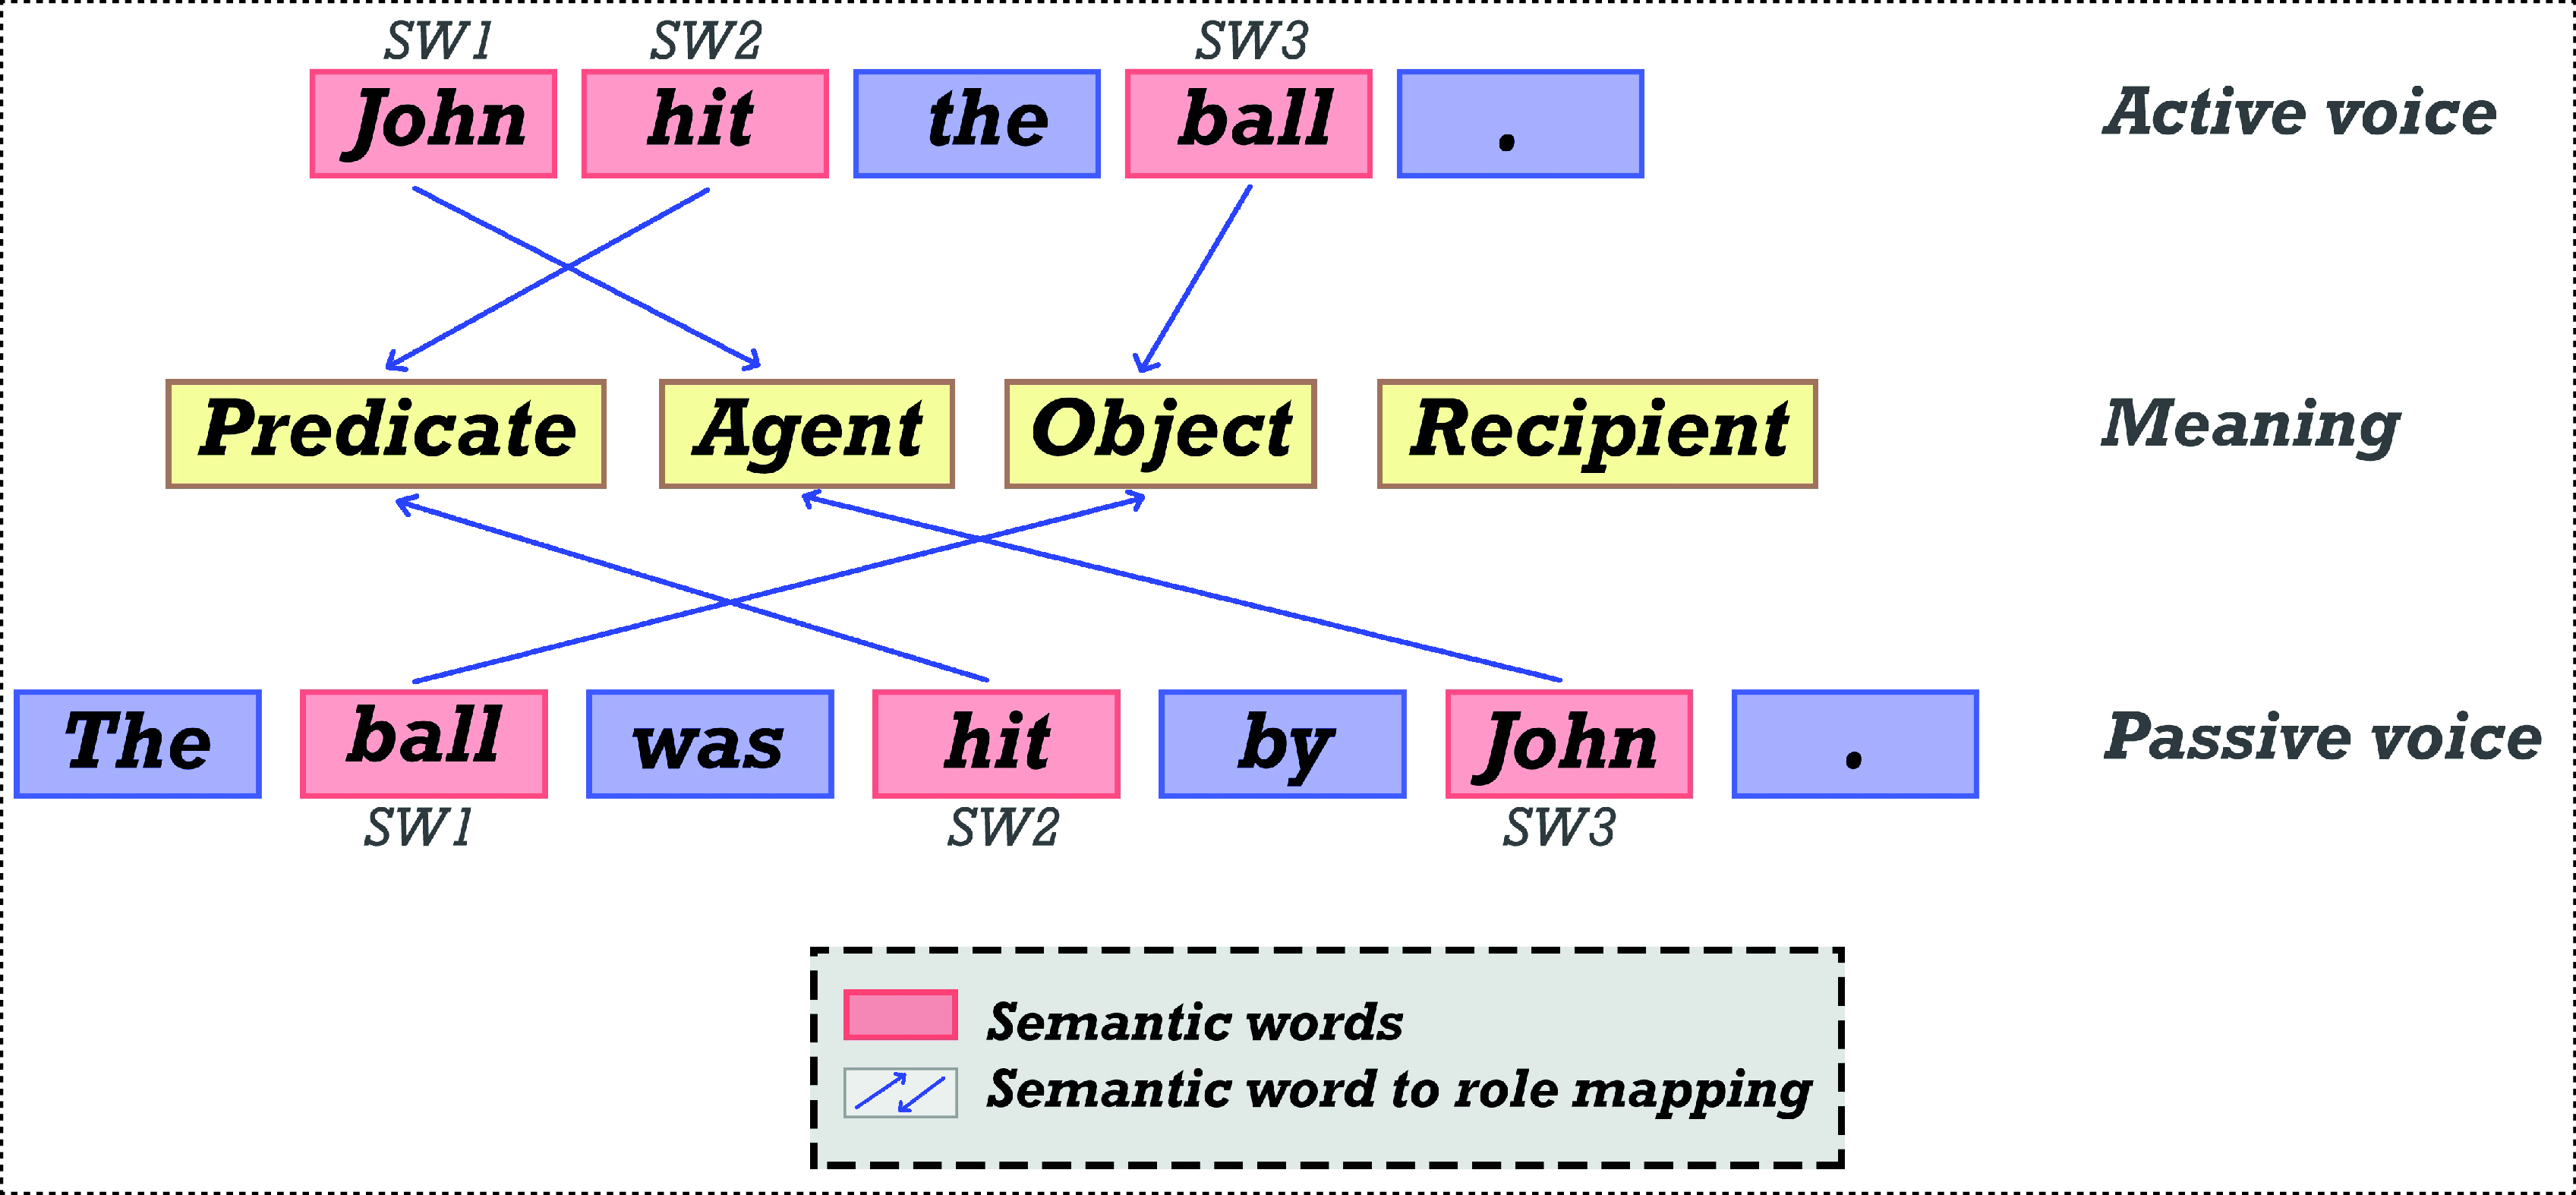
\includegraphics[width=0.8\linewidth,height=3.5cm, keepaspectratio]{grammatical_construction}
\caption[Word2vec semantic regularities]{\textbf{Word2vec semantic regularities.}} 
\label{fig:tra_gc}
\end{figure}

\begin{table}[hbtp]
\centering
\caption[Localist vector representation of sentence]{Transformation of a sentence by replacing semantic words with 'SW' token and localist vector representation of words used as an input for a sentence.}
\begin{tabular}{|c|c|c|c|c|c|c|c|}
\hline
\textbf{Original words} & \textbf{Transformed words}  & \multicolumn{6}{c|}{\textbf{Localist vectors}} \\ \hline
put		&	SW     & 0   & 1  & 0  & 1  & 0  & 1  \\ \hline
the		&	the    & 0   & 0  & 1  & 0  & 0  & 0  \\ \hline
ball	&	SW     & 0   & 1  & 0  & 1  & 0  & 1  \\ \hline
on		&	on     & 0   & 0  & 0  & 0  & 1  & 0  \\ \hline
the		&	the    & 0   & 0  & 1  & 0  & 0  & 0  \\ \hline
box		&	SW     & 0   & 1  & 0  & 1  & 0  & 1  \\ \hline
\end{tabular}
\label{tab:localist_representation}
\end{table}

\begin{figure}[hbtp]
\centering
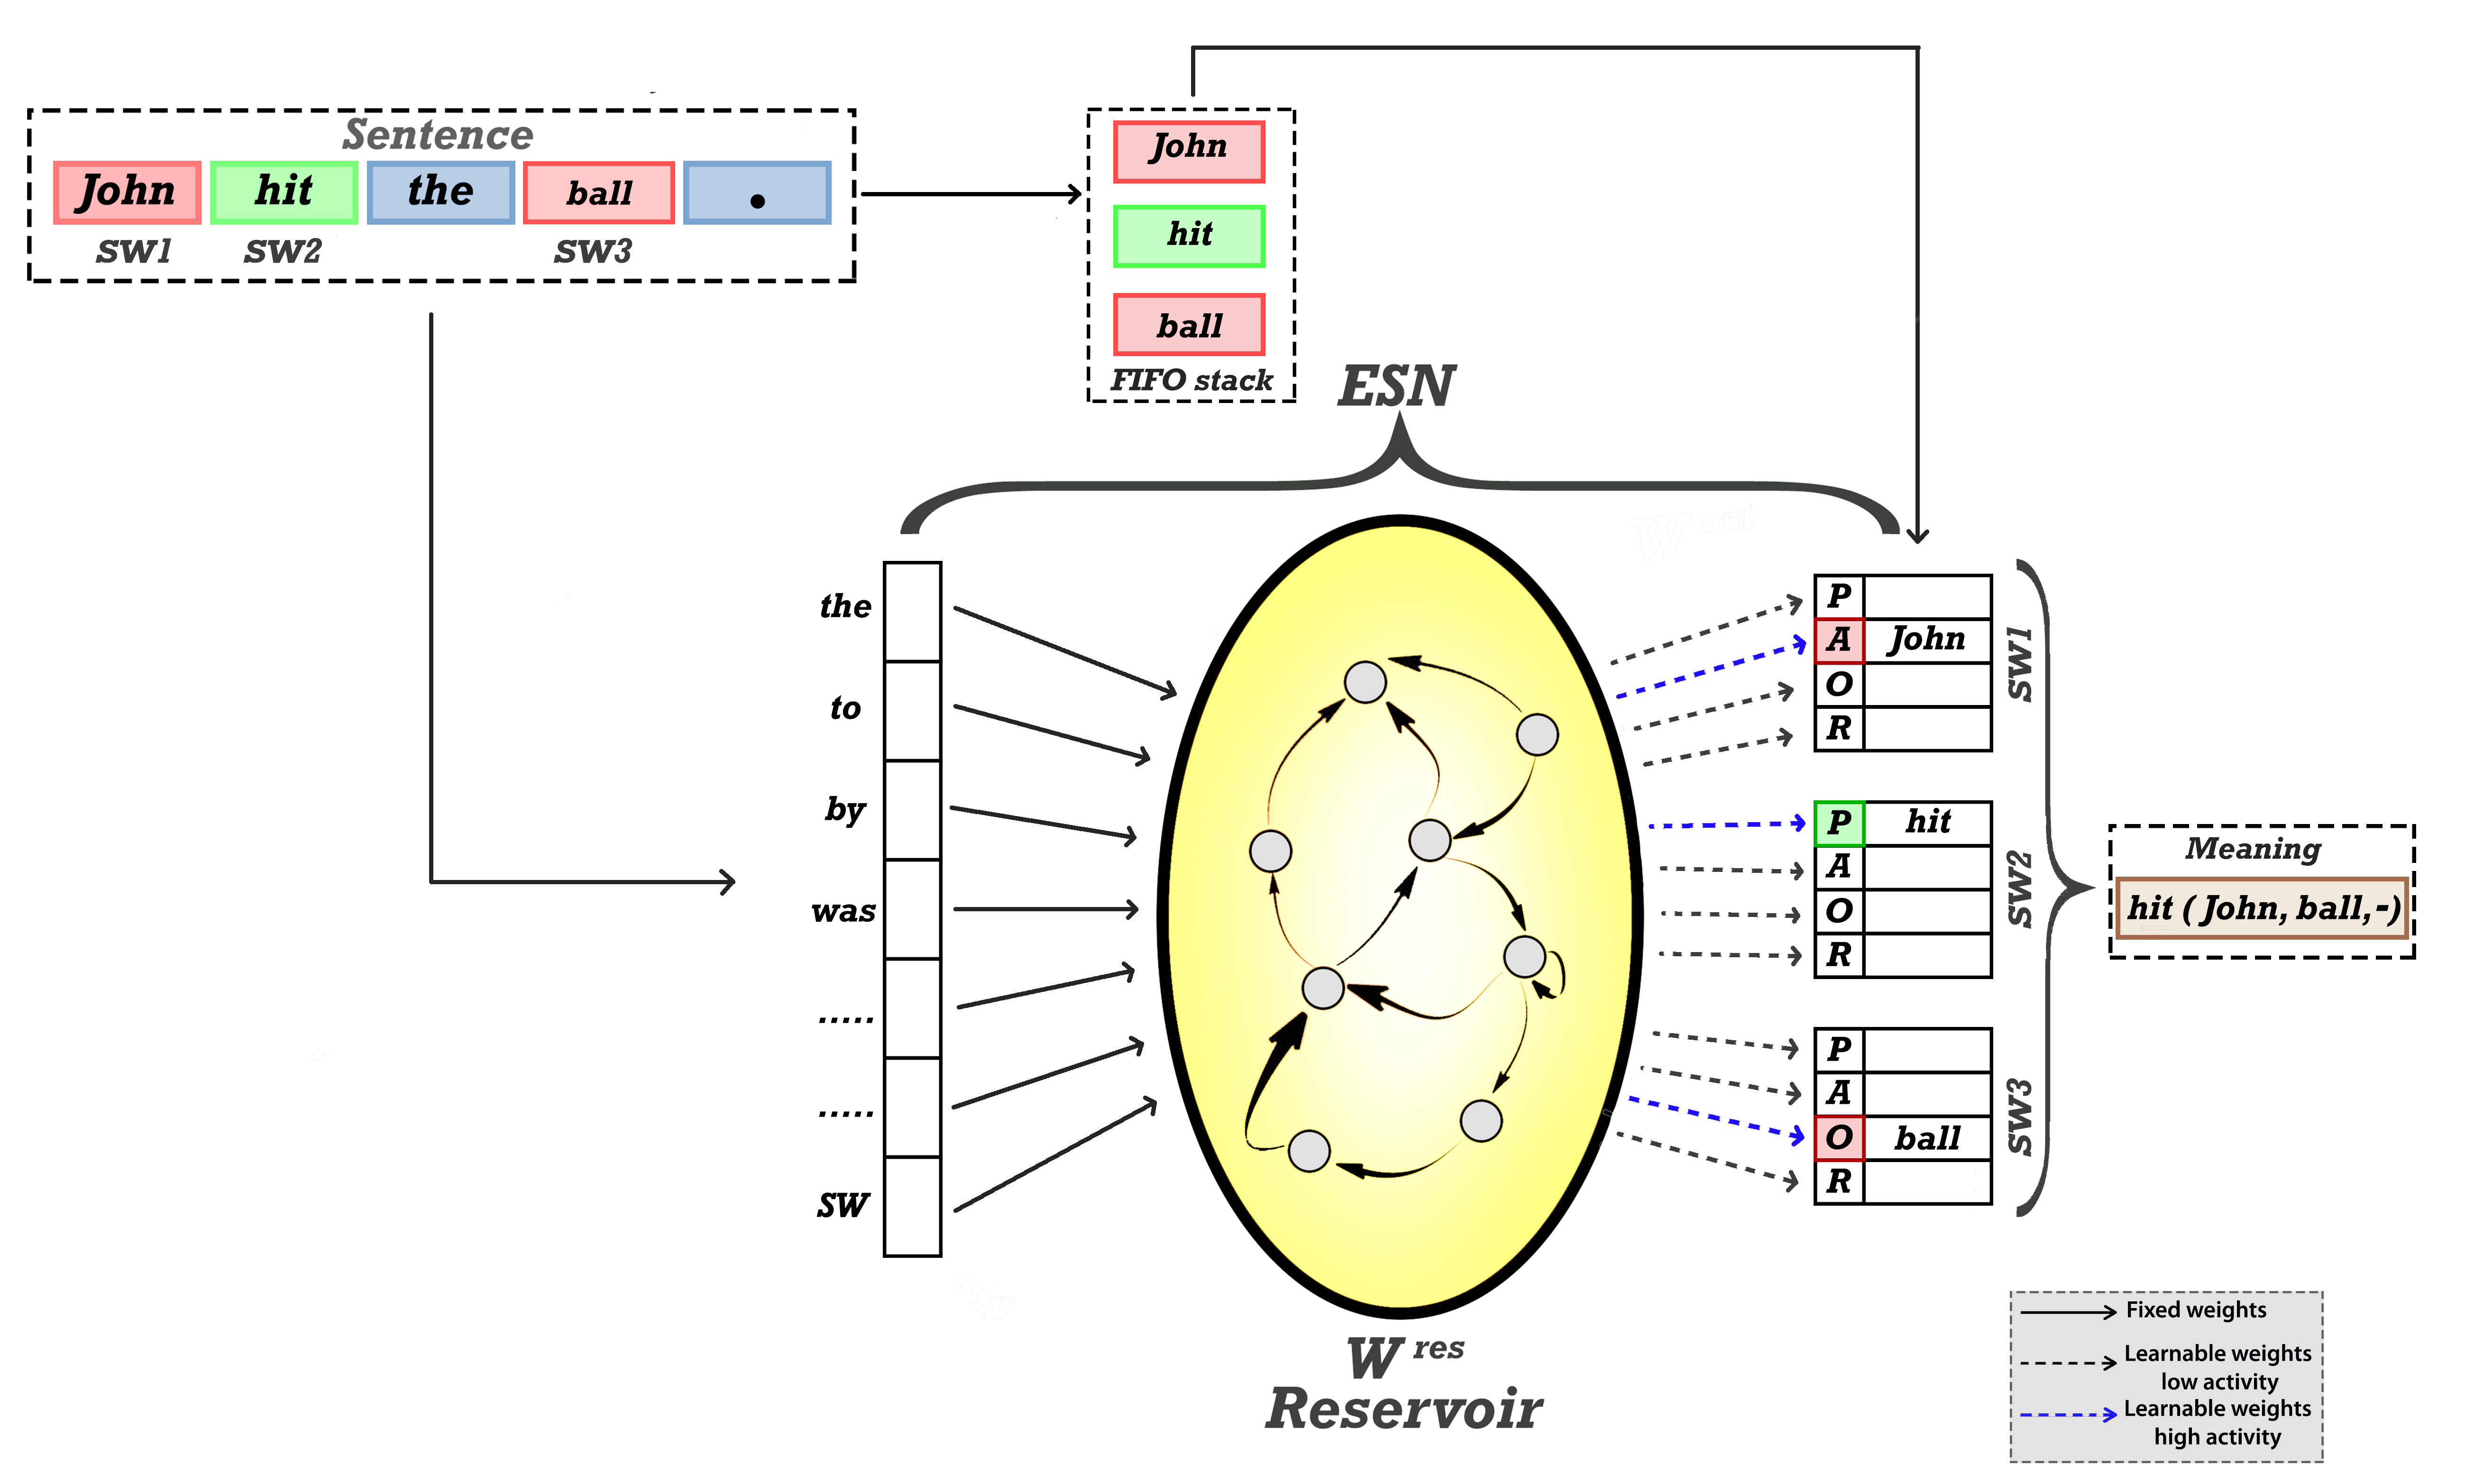
\includegraphics[width=0.8\linewidth]{xavier_model}
\caption[Word2vec semantic regularities]{\textbf{Word2vec semantic regularities.}} 
\label{fig:xavier_model}
\end{figure}

Thus for training the transformed sentences were presented to the model sequentially, word-by-word. Considering each word as a discrete atomic symbol, the words were encoded using localist vector representation, where all elements except the current input are zeros (see table \ref{tab:localist_representation}). Figure \ref{fig:xavier_model} shows the functional organization of the model. The localist word vectors are projected on the input layer of ESN and coded meaning of the input sentence is teacher-forced on the output layer of ESN. The model learns the thematic roles of all semantic words by learning reservoir to readout weights of ESN. During the testing the model predicts the coded meaning of the test sentence. The output activation is decoded to its meaning by thresholding the activation at last time step. For each SW word the that has highest activation is considered as the role of SW. Each semantic word in the memory stack is then mapped to the corresponding role (see fig. \ref{fig:xavier_model}). 

\subsection{Limitation of $\theta RARes$ model }

Transforming a sentence into its abstract representation (explained above) and using localist representation of each word in a sentence as an input to an ESN does not allow the network to leverage the information retrieved from semantically related words. The limitations for such an input representation mainly occurs with the ambiguous sentences. A sentence is said to be ambiguous if it has the same grammatical construction but different coded meaning and actual meaning. The limitation can be described below in the two ambiguous examples.

\paragraph{Example 1: Ambiguous Sentences}

\begin{enumerate}[noitemsep]
\item take (SW-1) the blue (SW-2) box (SW-3) \label{eg-1:sent-1}
\item take (SW-1) the left (SW-2) box (SW-3) \label{eg-1:sent-2}
\item throw(SW-1) the green(SW-2) box(SW-3)  \label{eg-1:sent-3} 
\end{enumerate}

All the three sentences having the same surface form after transforming the sentence by replacing the semantic words with 'SW' token i.e. SW the SW the SW SW.

\paragraph{Training with Sentence \ref{eg-1:sent-1}:} In the Sentence \ref{eg-1:sent-1} there are three semantic words namely SW-1: take, SW-2: blue, SW-3: box. During the training the sentence is input to the model from left to right word by word at each time step. The teacher output (thematic roles) of each semantic word is also teacher-forced as described below where, A: Action, O: Object, C: Color, I: Indicator. During the training ESN learns that second semantic word represents a \textit{'Color'}.

\begin{table}[hbtp]
\centering
\begin{minipage}{1.5in}
\begin{tabular}{|c|c|c|c|}
\hline
\multicolumn{4}{|c|}{\textbf{SW-1}}   \\ \hline
\textit{\textbf{A}}    & O & C & I 	\\ \hline
\textit{\textbf{take}} &   &   &  		\\  \hline
\end{tabular}
\end{minipage}
\begin{minipage}{1.5in}
\begin{tabular}{|c|c|c|c|}
\hline
\multicolumn{4}{|c|}{\textbf{SW-2}}                    \\ \hline
A	& O & \textit{\textbf{C}}    & I  \\ \hline
	&   & \textit{\textbf{blue}} & 	\\ \hline
\end{tabular}
\end{minipage}
\begin{minipage}{1.5in}
\begin{tabular}{|c|c|c|c|}
\hline
\multicolumn{4}{|c|}{\textbf{SW-3}}                                  \\ \hline
A	& \textit{\textbf{O}}   & C	& I \\ \hline
 	& \textit{\textbf{box}} &  	&   \\ \hline
\end{tabular}
\end{minipage}
\end{table}

\paragraph{Training with Sentence \ref{eg-1:sent-2}:} In the Sentence \ref{eg-1:sent-2} we have three semantic words; SW-1: take, SW-2: left, SW-3: ball. Both the sentences (\ref{eg-1:sent-1} and \ref{eg-1:sent-2}) differs only in the second semantic word. Now suppose we train this sentence with a teacher output as follows where symbols A, O, C and I have the same meaning as described above.

\begin{table}[hbtp]
\centering
\begin{minipage}{1.5in}
\begin{tabular}{|c|c|c|c|}
\hline
\multicolumn{4}{|c|}{\textbf{SW-1}}   \\ \hline
\textit{\textbf{A}}    & O & C & I \\ \hline
\textit{\textbf{take}} &   &   &  \\  \hline
\end{tabular}
\end{minipage}
\begin{minipage}{1.5in}
\begin{tabular}{|c|c|c|c|}
\hline
\multicolumn{4}{|c|}{\textbf{SW-2}}                    \\ \hline
A       & O & C    & \textit{\textbf{I}} \\ \hline
 &   &  & \textit{\textbf{left}} \\ \hline
\end{tabular}
\end{minipage}
\begin{minipage}{1.5in}
\begin{tabular}{|c|c|c|c|}
\hline
\multicolumn{4}{|c|}{\textbf{SW-3}}                                  \\ \hline
A                  & \textit{\textbf{O}}   & C                  & I \\ \hline
 & \textit{\textbf{box}} & \textit{\textbf{}} &   \\ \hline
\end{tabular}
\end{minipage}
\end{table}

As both the sentences used for training have the same surface form, the ESN learning from the sentence \ref{eg-1:sent-1} is disrupted after training with sentence \ref{eg-1:sent-2}. This is because the second semantic word in the sentence \ref{eg-1:sent-2} is trained to be an \textit{'Indicator'} whereas it was trained for \textit{'Color'} in the sentence \ref{eg-1:sent-1}. Such kind of ambiguous examples having the same surface form but different coded meaning (roles assignment) and actual meaning, drops the learning ability of the model. We believe that this problem is mainly because each input words are treated as a discrete atomic symbols, which does not carry any semantic information about the input words.

\paragraph{Testing with Sentence \ref{eg-1:sent-3}:} Now, when we use the sentence \ref{eg-1:sent-3} for testing, the network suggests two pseudo probabilities for the second semantic word \textit{'green'} i.e. being an \textit{'Indicator'} and a \textit{'Color'} as shown below. It becomes difficult for the model to resolve this ambiguity and assign the appropriate role. Although the word \textit{'green'} in the test sentence \ref{eg-1:sent-3} and the word \textit{'blue'} in the training sentence \ref{eg-1:sent-1} are semantically related i.e. both are colors. The model was not able to utilize this information as words were input to the in discrete forms for training. Thus by using localist vector representation we are depriving the ESN from the semantic information carried out by a words in a language.

\begin{table}[hbtp]
\centering
\begin{minipage}{1.5in}
\begin{tabular}{|c|c|c|c|}
\hline
\multicolumn{4}{|c|}{\textbf{SW-2}}  \\ \hline
A	& O & \textit{\textbf{C(0.5)}}   & \textit{\textbf{I(0.5)}} \\ \hline
	&   & \textit{\textbf{green}} 	  & \textit{\textbf{green}} \\ \hline
\end{tabular}
\end{minipage}
\end{table}

\noindent Similary the following three sentences also have the same suface form i.e. The SW is SW to SW.

\begin{enumerate}[noitemsep,label=(\roman*)]
\item The chicken(SW-1) is cooked(SW-2) to eat(SW-3) \label{eg-1:sent-i}
\item The ball(SW-1) is given(SW-2) to John(SW-3) \label{eg-1:sent-ii}
\item The book(SW-1) is taken(SW-2) to John(SW-3) \label{eg-1:sent-iii}
\end{enumerate}

Clearly we can see that the third semantic word is a \textit{'predicate'} in Sentence \ref{eg-1:sent-i} and \textit{'noun'} in sentence \ref{eg-1:sent-ii}. Thus if network is trained on sentences \ref{eg-1:sent-i} and \ref{eg-1:sent-ii} and tested on sentence \ref{eg-1:sent-iii} the network is not able to resolve the ambiguity for semantic word SW-3, which possibly leads to wrong labelling of this word.

\paragraph{Example 2: Ambiguous and Polysemous Sentences}

\begin{enumerate}[noitemsep]
\item John (SW-1) books (SW-2) the ticket (SW-3) to London (SW-4) \label{eg-2:sent-1}
\item John (SW-1) read (SW-2) the books (SW-3) to learn (SW-4) \label{eg-2:sent-2}
\end{enumerate}

Both the above sentences share the same surface form i.e. SW SW the SW to SW.

\paragraph{Training model on sentence \ref{eg-2:sent-1}} Training the model on the first sentence, the fourth semantic word \textit{'London'} is trained to be as a \textit{location}.

\paragraph{Testing model on sentence \ref{eg-2:sent-2}} Testing the model with the second sentence, the fourth semantic word \textit{learn} will be assigned the role of a location (as network was trained for this only) whereas it is actually a \textit{predicate}. The reason for such problem is that each semantic word is considered as an unique token without taking into consideration semantics of an individual word. Hence the network could not exploit the semantic information of the words during the role assignment.

\paragraph{Issue with Polysemous words:} In the first sentence, the second semantic word \textit{books} is the predicate and describe the action of making reservation, whereas the same word (books) in the second sentence is an \textit{'object'}, and represents a book which we read. Although both words are same but they represent different meanings depending on the context. These kind of words with different meaning are also known as \textit{polysemous} words. Semantic ambiguities because of polysemous words is hard to resolve with localist vector representation where each word is treated as an unique identifier. To resolve such kind of semantic ambiguities, distributed embedding of words can be useful as they are learned using the the contextual information of words.

\subsection{Research Hypothesis}

Use of abstract form of sentence and localist word vectors as an input to the ESN have produced the promising results for the thematic role assignment task\cite{xavier:2013:RT, tra:xavier_wermter:2014}. But the behaviour of the model with the distributed word embeddings was left unexplored. Thus we hypothesize that using the distributed word embeddings (e.g. Word2Vec word embeddings) could possibly resolve the problems described in the above mentioned two examples by taking into consideration the fact that they capture and encode semantic and syntactic information of words \cite{w2v:mikolov_2013_distributed, w2v:regularities_in_word_representations}. Another advantage of distributed word embedding observed over localist vector representation is that the multidimensional distributed vector representation of semantically related words remains close in neighborhood within words embedding space (see Fig. 3). This could possibly allow the model to learn this dynamics from the distributed representation of the words and avoid the disruption caused by semantically unrelated words (as in Example 1) in the sentences with the same grammatical constructions. Whereas this semantic grouping of words is not possible in localist vector encoding as words are represented as discrete atomic symbols.

Consider using distributed embedding of words for both the sentences in Example 2. The distributed embedding of the word \textit{'London'} (sentence 1, Example 2) encodes that it represents a \textit{'location'} along with several other semantic information. Similarly, the distributed embedding of word \textit{'learn'} (sentence 2, Example 2) also encodes that it is a \textit{'predicate'} along with other semantic information. When these distributed embedding is used as an input to train the network, the learning of the model may not be disrupted by the sentences having the same surface form, but different semantic words. This is because, the semantic information about the word is exposed to network and learned by it. Hence, thematic roles could be assigned to the words more accurately although the sentence have the same surface form.
